\documentclass[10pt,fleqn]{beamer}
\usepackage[utf8]{inputenc}
\usepackage[T1]{fontenc}
\usepackage{ae,aecompl}
% for double screen presentation
%\usepackage{pgfpages}
%\setbeamertemplate{note page}[sqeeze]
%\setbeameroption{show notes on second screen=right}

\usepackage{float}
\usepackage{booktabs}
\usepackage{multirow}
\usepackage{sansmathfonts}
\usepackage{amsmath,times,empheq}
\usepackage{fontawesome} % itemize symbols
%\title{Visualization V1}
%\date{}
%\author[Hélder]{\underline{Hélder C. Barbosa}, Ricardo Costa, Gaspar J. Machado}
%\institute{\parbox{\linewidth}{\centering%
%Centre of Mathematics, University of Minho, Guimarães, Portugal\endgraf\bigskip\tiny{
%Financed by National Funds and by FCT within the Project FCT - UID/MAT/00013/2013}}}

\usetheme{texsx}

%\usefonttheme[onlymath]{serif}
%\usefonttheme{serif}
%\usefonttheme{professionalfonts}

\usepackage{empheq}
\newcommand{\MatR}[2]{{\cal M}_{#1\times #2}(\mathbb R)}
\newcommand{\VarCount}[3]{#1=#2,\ldots,#3}

\begin{document}
 
%---------------------------------------------------
%\begin{frame}[noframenumbering]
%\titlepage
%\end{frame}
%\note{
%}
%---------------------------------------------------


 
\section{Pure Diffusion}

%%---------------------------------------------------
\begin{frame}
\frametitle{Pure Diffusion | Formulation}

\[
\begin{cases}
-\psi''=s & \text{ in}\quad  \Omega=]x_\text{lf},x_\text{rg}+\epsilon[\\
\psi=\psi_{\text{lf},0} & \text{ on}\quad  x=x_\text{lf}\\
-\psi'=\psi_{\text{rg},1} & \text{ on}\quad  x=x_\text{rg}+\epsilon
\end{cases}
\]

\end{frame}
%%---------------------------------------------------

%-------------------------------------------------
\begin{frame}
\frametitle{Mesh}

\begin{center}
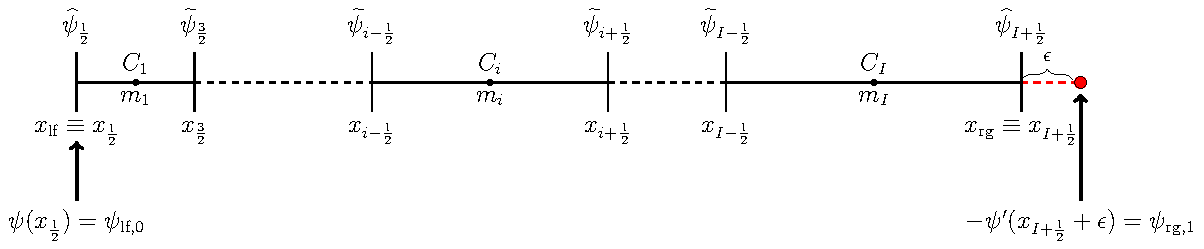
\includegraphics[width=\textwidth]{images/mesh_notation_reconstructions/mesh_notation_reconstructions}
\end{center}

\begin{itemize}
\item $C_i$ --- cell $i$
\item $I$ --- number of cells
\item $x_{i-\frac{1}{2}}$, $x_{i+\frac{1}{2}}$ --- boundary points of cell $i$
\item $h_i$ --- length of cell $i$
\item $m_i$ --- centroid of cell $i$
\end{itemize}

\end{frame}
%-------------------------------------------------

%---------------------------------------------------
\begin{frame}
\frametitle{Polynomial Reconstructions | Inner Vertices}

\[
\psi_{i+\frac{1}{2},\mathsf{d}}(x)=\sum_{\alpha=0}^\mathsf{d} \mathcal R_{i+\frac{1}{2},\alpha}(x-x_{i+\frac{1}{2}})^\alpha
\]
\begin{align*}
\min_{\mathcal R_{i+\frac{1}{2},0},\ldots,\mathcal R_{i+\frac{1}{2},\mathsf d}} & \quad
\sum_{j\in\widehat S_{i+\frac{1}{2}}} \omega_j\left [\frac{1}{h_j} \int_{c_j} \psi_{i+\frac{1}{2},\mathsf{d}}(x)\mathsf dx -\psi_j \right]^2
\end{align*}

This will be needed to approximate $\mathbf{F}_{i+\frac{1}{2}}\approx\mathcal{F}_{i+\frac{1}{2}}= \widetilde \psi'_{i+\frac{1}{2}}(x_{i+\frac{1}{2}})$

\end{frame}
%---------------------------------------------------

%---------------------------------------------------
\begin{frame}
\frametitle{Polynomial Reconstructions | Left Boundary}

\[
\psi_{\frac{1}{2},\mathsf{d}}(x)=\sum_{\alpha=0}^\mathsf{d} \mathcal R_{\frac{1}{2},\alpha}(x-x_{\text{lf}})^\alpha
\]
\begin{align*}
\min_{\mathcal R_{\frac{1}{2},0},\ldots,\mathcal R_{\frac{1}{2},\mathsf d}} & \quad
\sum_{j\in\widehat S_\frac{1}{2}} \omega_j\left [\frac{1}{h_j} \int_{c_j} \psi_{\frac{1}{2},\mathsf{d}}(x)\mathsf dx -\psi_j \right]^2\\
\text{s.t.} & \quad \psi_{\frac{1}{2},\mathsf{d}}(x_{\text{lf}})=\psi_{\text{lf},0}
\end{align*}

This will be needed to approximate $\mathbf{F}_{\frac{1}{2}}\approx\mathcal{F}_{\frac{1}{2}} = \psi'_{\frac{1}{2}}(x_{\text{lf}})$
\end{frame}
%---------------------------------------------------

%---------------------------------------------------
\begin{frame}
\frametitle{Polynomial Reconstructions | Right Boundary}

\[
\psi_{I+\frac{1}{2},\mathsf{d}}(x)=\sum_{\alpha=0}^\mathsf{d} \mathcal R_{I+\frac{1}{2},\alpha}(x-x_{\text{rg}})^\alpha
\]
\begin{align*}
\min_{\mathcal R_{I+\frac{1}{2},0},\ldots,\mathcal R_{I+\frac{1}{2},\mathsf d}} & \quad
\sum_{j\in\widehat S_{I+\frac{1}{2}}} \omega_j\left [\frac{1}{h_j} \int_{c_j} \psi_{I+\frac{1}{2},\mathsf{d}}(x)\mathsf dx -\psi_j \right]^2\\
\text{s.t.} & \quad -\psi'_{I+\frac{1}{2},\mathsf{d}}(x_{\text{rg}}+\epsilon)=\psi_{\text{rg},1}
\end{align*}

This will be needed to approximate $\mathbf{F}_{I+\frac{1}{2}}\approx\mathcal{F}_{I+\frac{1}{2}}=\widehat \psi'_{I+\frac{1}{2}}(x_{\text{rg}})$
\end{frame}
%---------------------------------------------------

%-------------------------------------------------
\begin{frame}
\frametitle{Tests}

In this test we will consider:
\begin{itemize}
\item $\overline{\Omega}=[0,1+\epsilon]$
\item $\psi(x)=\exp(x)$
\item $\psi(0)=1$
\item $\varphi_{\text{n2}}=-\exp(1+\epsilon)$
%\item $\psi(1+\epsilon)=-\exp(1+\epsilon)$
\end{itemize}
\end{frame}
%-------------------------------------------------

%-------------------------------------------------
\begin{frame}
\frametitle{Tests | $\epsilon=0$ | degree d}

\begin{minipage}[b]{0.49\textwidth}
\small
\centering 
uniform mesh
\begin{table}[H]
\centering
\resizebox*{!}{\dimexpr\textheight-6\baselineskip\relax}{%
\begin{tabular}{@{}l c c c@{}}
\toprule
 & $I$ & E$_{0,\infty}$ & O$_{0,\infty}$\\
\midrule
\multirow{4}{*}{$\mathbb{P}_{1}$}
 & 10 & 1.09E$-$02 & ---\\
 & 20 & 2.68E$-$03 & 2.02 \\
 & 30 & 1.19E$-$03 & 2.01 \\
 & 40 & 6.67E$-$04 & 2.01 \\
\midrule
\multirow{4}{*}{$\mathbb{P}_{2}$}
 & 10 & 4.93E$-$03 & ---\\
 & 20 & 1.38E$-$03 & 1.83 \\
 & 30 & 8.01E$-$04 & 1.35 \\
 & 40 & 3.88E$-$04 & 2.52 \\
\midrule
\multirow{4}{*}{$\mathbb{P}_{3}$}
 & 10 & 2.99E$-$05 & ---\\
 & 20 & 1.93E$-$06 & 3.95 \\
 & 30 & 3.86E$-$07 & 3.97 \\
 & 40 & 1.23E$-$07 & 3.98 \\
\midrule
\multirow{4}{*}{$\mathbb{P}_{4}$}
 & 10 & 1.15E$-$05 & ---\\
 & 20 & 1.20E$-$06 & 3.26 \\
 & 30 & 2.00E$-$07 & 4.42 \\
 & 40 & 6.69E$-$08 & 3.80 \\
\midrule
\multirow{4}{*}{$\mathbb{P}_{5}$}
 & 10 & 9.53E$-$08 & ---\\
 & 20 & 2.00E$-$09 & 5.58 \\
 & 30 & 1.91E$-$10 & 5.79 \\
 & 40 & 3.53E$-$11 & 5.86 \\
\bottomrule
\end{tabular}}
\end{table}

\end{minipage}
\begin{minipage}[b]{0.49\textwidth}
\small
\centering 
non-uniform mesh
\begin{table}[H]
\small
\centering
\resizebox*{!}{\dimexpr\textheight-6\baselineskip\relax}{%
\begin{tabular}{@{}l c c c@{}}
\toprule
 & $I$ & E$_{0,\infty}$ & O$_{0,\infty}$\\
\midrule
\multirow{4}{*}{$\mathbb{P}_{1}$}
 & 10 & 2.18E$-$02 & ---\\
 & 20 & 5.50E$-$03 & 1.99 \\
 & 30 & 2.56E$-$03 & 1.88 \\
 & 40 & 1.60E$-$03 & 1.64 \\
\midrule
\multirow{4}{*}{$\mathbb{P}_{2}$}
 & 10 & 4.28E$-$03 & ---\\
 & 20 & 2.05E$-$03 & 1.06 \\
 & 30 & 1.70E$-$03 & 0.45 \\
 & 40 & 4.96E$-$04 & 4.29 \\
\midrule
\multirow{4}{*}{$\mathbb{P}_{3}$}
 & 10 & 4.11E$-$05 & ---\\
 & 20 & 2.29E$-$06 & 4.16 \\
 & 30 & 7.21E$-$07 & 2.85 \\
 & 40 & 1.76E$-$07 & 4.91 \\
\midrule
\multirow{4}{*}{$\mathbb{P}_{4}$}
 & 10 & 1.07E$-$05 & ---\\
 & 20 & 8.77E$-$07 & 3.61 \\
 & 30 & 2.26E$-$07 & 3.34 \\
 & 40 & 6.37E$-$08 & 4.40 \\
\midrule
\multirow{4}{*}{$\mathbb{P}_{5}$}
 & 10 & 7.38E$-$07 & ---\\
 & 20 & 1.01E$-$08 & 6.20 \\
 & 30 & 1.05E$-$09 & 5.58 \\
 & 40 & 2.04E$-$10 & 5.69 \\
\bottomrule
\end{tabular}}
\end{table}

\end{minipage}
\end{frame}
%-------------------------------------------------

%-------------------------------------------------
\begin{frame}
\frametitle{Tests | $\epsilon=\frac{h}{2}$ | degree d}

\begin{minipage}[b]{0.49\textwidth}
\small
\centering 
uniform mesh
\begin{table}[H]
\centering
\resizebox*{!}{\dimexpr\textheight-6\baselineskip\relax}{%
\begin{tabular}{@{}l c c c@{}}
\toprule
 & $I$ & E$_{0,\infty}$ & O$_{0,\infty}$\\
\midrule
\multirow{4}{*}{$\mathbb{P}_{1}$}
 & 10 & 1.22E$-$01 & ---\\
 & 20 & 6.44E$-$02 & 0.92 \\
 & 30 & 4.37E$-$02 & 0.95 \\
 & 40 & 3.31E$-$02 & 0.97 \\
\midrule
\multirow{4}{*}{$\mathbb{P}_{2}$}
 & 10 & 5.10E$-$03 & ---\\
 & 20 & 8.54E$-$04 & 2.58 \\
 & 30 & 4.07E$-$04 & 1.83 \\
 & 40 & 1.33E$-$04 & 3.89 \\
\midrule
\multirow{4}{*}{$\mathbb{P}_{3}$}
 & 10 & 1.33E$-$04 & ---\\
 & 20 & 1.02E$-$05 & 3.70 \\
 & 30 & 2.16E$-$06 & 3.83 \\
 & 40 & 7.08E$-$07 & 3.88 \\
\midrule
\multirow{4}{*}{$\mathbb{P}_{4}$}
 & 10 & 1.62E$-$05 & ---\\
 & 20 & 9.43E$-$07 & 4.10 \\
 & 30 & 9.41E$-$08 & 5.69 \\
 & 40 & 2.36E$-$08 & 4.81 \\
\midrule
\multirow{4}{*}{$\mathbb{P}_{5}$}
 & 10 & 3.29E$-$07 & ---\\
 & 20 & 6.16E$-$09 & 5.74 \\
 & 30 & 5.75E$-$10 & 5.85 \\
 & 40 & 1.06E$-$10 & 5.89 \\
\bottomrule
\end{tabular}}
\end{table}

\end{minipage}
\begin{minipage}[b]{0.49\textwidth}
\small
\centering 
non-uniform mesh
\begin{table}[H]
\caption{Numerical results of PRO1 scheme for $\phi(x)=\exp(x)$, $\kappa(x)=1$, and $u(x)=0$.}
\setlength{\tabcolsep}{5pt}
\centering
\begin{tabular}{@{}l c c c c c@{}}
\toprule
 &  & \multicolumn{2}{c}{PRO1} & \multicolumn{2}{c}{PRO2}\\
\midrule
 & $I$ & E$_{0,I}(E_{\infty})$ & E$_{0,I}(O_{\infty})$ & E$_{0,I}(E_{\infty})$ & E$_{0,I}(O_{\infty})$\\
\midrule
\multirow{4}{*}{$\mathbb{P}_{1}$}
 & 10 & 1.22E$-$01 & --- & 1.22E$-$01 & ---\\
 & 20 & 6.44E$-$02 & 0.92 & 6.44E$-$02 & 0.92 \\
 & 30 & 4.37E$-$02 & 0.95 & 4.37E$-$02 & 0.95 \\
 & 40 & 3.30E$-$02 & 0.98 & 3.30E$-$02 & 0.98 \\
\midrule
\multirow{4}{*}{$\mathbb{P}_{2}$}
 & 10 & 4.58E$-$03 & --- & 4.58E$-$03 & ---\\
 & 20 & 2.19E$-$03 & 1.07 & 2.19E$-$03 & 1.07 \\
 & 30 & 1.83E$-$03 & 0.44 & 1.83E$-$03 & 0.44 \\
 & 40 & 1.46E$-$04 & 8.79 & 1.46E$-$04 & 8.79 \\
\midrule
\multirow{4}{*}{$\mathbb{P}_{3}$}
 & 10 & 6.19E$-$05 & --- & 6.19E$-$05 & ---\\
 & 20 & 5.52E$-$06 & 3.49 & 5.52E$-$06 & 3.49 \\
 & 30 & 7.02E$-$07 & 5.09 & 7.02E$-$07 & 5.09 \\
 & 40 & 2.41E$-$07 & 3.72 & 2.41E$-$07 & 3.72 \\
\midrule
\multirow{4}{*}{$\mathbb{P}_{4}$}
 & 10 & 6.79E$-$06 & --- & 6.79E$-$06 & ---\\
 & 20 & 3.29E$-$07 & 4.37 & 3.29E$-$07 & 4.37 \\
 & 30 & 5.89E$-$08 & 4.25 & 5.89E$-$08 & 4.25 \\
 & 40 & 1.03E$-$08 & 6.07 & 1.03E$-$08 & 6.07 \\
\midrule
\multirow{4}{*}{$\mathbb{P}_{5}$}
 & 10 & 5.66E$-$07 & --- & 5.66E$-$07 & ---\\
 & 20 & 8.38E$-$09 & 6.08 & 8.38E$-$09 & 6.08 \\
 & 30 & 9.61E$-$10 & 5.34 & 9.61E$-$10 & 5.34 \\
 & 40 & 1.87E$-$10 & 5.68 & 1.87E$-$10 & 5.68 \\
\bottomrule
\end{tabular}
\label{Table:PRO:Test1}
\end{table}

\end{minipage}
\end{frame}
%-------------------------------------------------

%-------------------------------------------------
\begin{frame}
\frametitle{Tests | $\epsilon=\frac{h}{2}$ | degree d+1}

\begin{minipage}[b]{0.49\textwidth}
\small
\centering 
uniform mesh
\begin{table}[H]
\centering
\resizebox*{!}{\dimexpr\textheight-6\baselineskip\relax}{%
\begin{tabular}{@{}l c c c@{}}
\toprule
 & $I$ & E$_{0,\infty}$ & O$_{0,\infty}$\\
\midrule
\multirow{4}{*}{$\mathbb{P}_{1}/\mathbb{P}_{2}$}
 & 10 & 9.06E$-$03 & ---\\
 & 20 & 2.28E$-$03 & 1.99 \\
 & 30 & 1.01E$-$03 & 2.00 \\
 & 40 & 5.71E$-$04 & 2.00 \\
\midrule
\multirow{4}{*}{$\mathbb{P}_{2}/\mathbb{P}_{3}$}
 & 10 & 2.36E$-$03 & ---\\
 & 20 & 3.87E$-$04 & 2.61 \\
 & 30 & 2.44E$-$04 & 1.14 \\
 & 40 & 6.54E$-$05 & 4.57 \\
\midrule
\multirow{4}{*}{$\mathbb{P}_{3}/\mathbb{P}_{4}$}
 & 10 & 1.91E$-$05 & ---\\
 & 20 & 1.14E$-$06 & 4.07 \\
 & 30 & 2.21E$-$07 & 4.04 \\
 & 40 & 6.94E$-$08 & 4.03 \\
\midrule
\multirow{4}{*}{$\mathbb{P}_{4}/\mathbb{P}_{5}$}
 & 10 & 5.81E$-$06 & ---\\
 & 20 & 5.99E$-$07 & 3.28 \\
 & 30 & 3.38E$-$08 & 7.09 \\
 & 40 & 7.70E$-$09 & 5.14 \\
\midrule
\multirow{4}{*}{$\mathbb{P}_{5}/\mathbb{P}_{6}$}
 & 10 & 1.50E$-$07 & ---\\
 & 20 & 2.73E$-$09 & 5.78 \\
 & 30 & 2.54E$-$10 & 5.86 \\
 & 40 & 4.64E$-$11 & 5.90 \\
\bottomrule
\end{tabular}}
\end{table}

\end{minipage}
\begin{minipage}[b]{0.49\textwidth}
\small
\centering 
non-uniform mesh
\begin{table}[H]
\centering
\resizebox*{!}{\dimexpr\textheight-6\baselineskip\relax}{%
\begin{tabular}{@{}l c c c@{}}
\toprule
 & $I$ & E$_{0,\infty}$ & O$_{0,\infty}$\\
\midrule
\multirow{4}{*}{$\mathbb{P}_{1}/\mathbb{P}_{2}$}
 & 10 & 2.02E$-$02 & ---\\
 & 20 & 5.28E$-$03 & 1.94 \\
 & 30 & 2.45E$-$03 & 1.89 \\
 & 40 & 1.46E$-$03 & 1.80 \\
\midrule
\multirow{4}{*}{$\mathbb{P}_{2}/\mathbb{P}_{3}$}
 & 10 & 3.29E$-$03 & ---\\
 & 20 & 2.15E$-$03 & 0.61 \\
 & 30 & 1.82E$-$03 & 0.40 \\
 & 40 & 1.30E$-$04 & 9.19 \\
\midrule
\multirow{4}{*}{$\mathbb{P}_{3}/\mathbb{P}_{4}$}
 & 10 & 4.21E$-$05 & ---\\
 & 20 & 2.34E$-$06 & 4.17 \\
 & 30 & 7.18E$-$07 & 2.92 \\
 & 40 & 1.77E$-$07 & 4.87 \\
\midrule
\multirow{4}{*}{$\mathbb{P}_{4}/\mathbb{P}_{5}$}
 & 10 & 5.24E$-$06 & ---\\
 & 20 & 2.05E$-$07 & 4.68 \\
 & 30 & 6.60E$-$08 & 2.79 \\
 & 40 & 1.22E$-$08 & 5.86 \\
\midrule
\multirow{4}{*}{$\mathbb{P}_{5}/\mathbb{P}_{6}$}
 & 10 & 5.45E$-$07 & ---\\
 & 20 & 8.16E$-$09 & 6.06 \\
 & 30 & 9.52E$-$10 & 5.30 \\
 & 40 & 1.86E$-$10 & 5.68 \\
\bottomrule
\end{tabular}}
\end{table}

\end{minipage}
\end{frame}
%-------------------------------------------------

%-------------------------------------------------
\begin{frame}
\frametitle{Tests | $\epsilon=h$ | degree d}

\begin{minipage}[b]{0.49\textwidth}
\small
\centering 
uniform mesh
\begin{table}[H]
\centering
\resizebox*{!}{\dimexpr\textheight-6\baselineskip\relax}{%
\begin{tabular}{@{}l c c c@{}}
\toprule
 & $I$ & E$_{0,\infty}$ & O$_{0,\infty}$\\
\midrule
\multirow{4}{*}{$\mathbb{P}_{1}$}
 & 10 & 2.61E$-$01 & ---\\
 & 20 & 1.33E$-$01 & 0.97 \\
 & 30 & 8.94E$-$02 & 0.98 \\
 & 40 & 6.73E$-$02 & 0.99 \\
\midrule
\multirow{4}{*}{$\mathbb{P}_{2}$}
 & 10 & 9.72E$-$03 & ---\\
 & 20 & 1.38E$-$03 & 2.81 \\
 & 30 & 5.72E$-$04 & 2.17 \\
 & 40 & 2.01E$-$04 & 3.64 \\
\midrule
\multirow{4}{*}{$\mathbb{P}_{3}$}
 & 10 & 1.78E$-$04 & ---\\
 & 20 & 1.30E$-$05 & 3.78 \\
 & 30 & 2.70E$-$06 & 3.87 \\
 & 40 & 8.78E$-$07 & 3.91 \\
\midrule
\multirow{4}{*}{$\mathbb{P}_{4}$}
 & 10 & 1.90E$-$05 & ---\\
 & 20 & 1.03E$-$06 & 4.20 \\
 & 30 & 1.05E$-$07 & 5.62 \\
 & 40 & 2.63E$-$08 & 4.82 \\
\midrule
\multirow{4}{*}{$\mathbb{P}_{5}$}
 & 10 & 4.00E$-$07 & ---\\
 & 20 & 7.42E$-$09 & 5.75 \\
 & 30 & 6.91E$-$10 & 5.86 \\
 & 40 & 1.27E$-$10 & 5.90 \\
\bottomrule
\end{tabular}}
\end{table}

\end{minipage}
\begin{minipage}[b]{0.49\textwidth}
\small
\centering 
non-uniform mesh
\begin{table}[H]
\centering
\resizebox*{!}{\dimexpr\textheight-6\baselineskip\relax}{%
\begin{tabular}{@{}l c c c@{}}
\toprule
 & $I$ & E$_{0,\infty}$ & O$_{0,\infty}$\\
\midrule
\multirow{4}{*}{$\mathbb{P}_{1}$}
 & 10 & 2.66E$-$01 & ---\\
 & 20 & 1.34E$-$01 & 0.98 \\
 & 30 & 9.01E$-$02 & 0.99 \\
 & 40 & 6.75E$-$02 & 1.00 \\
\midrule
\multirow{4}{*}{$\mathbb{P}_{2}$}
 & 10 & 5.97E$-$03 & ---\\
 & 20 & 2.26E$-$03 & 1.40 \\
 & 30 & 1.84E$-$03 & 0.51 \\
 & 40 & 1.90E$-$04 & 7.89 \\
\midrule
\multirow{4}{*}{$\mathbb{P}_{3}$}
 & 10 & 8.01E$-$05 & ---\\
 & 20 & 6.90E$-$06 & 3.54 \\
 & 30 & 7.87E$-$07 & 5.35 \\
 & 40 & 2.99E$-$07 & 3.37 \\
\midrule
\multirow{4}{*}{$\mathbb{P}_{4}$}
 & 10 & 8.09E$-$06 & ---\\
 & 20 & 3.70E$-$07 & 4.45 \\
 & 30 & 5.78E$-$08 & 4.58 \\
 & 40 & 1.09E$-$08 & 5.80 \\
\midrule
\multirow{4}{*}{$\mathbb{P}_{5}$}
 & 10 & 5.69E$-$07 & ---\\
 & 20 & 8.42E$-$09 & 6.08 \\
 & 30 & 9.63E$-$10 & 5.35 \\
 & 40 & 1.88E$-$10 & 5.69 \\
\bottomrule
\end{tabular}}
\end{table}

\end{minipage}
\end{frame}
%-------------------------------------------------

%-------------------------------------------------
\begin{frame}
\frametitle{Tests | $\epsilon=h$ | degree d+1}

\begin{minipage}[b]{0.315\textwidth}
\small
\centering 
uniform mesh
\begin{table}[H]
\caption{Numerical results of PRO1 scheme for $\phi(x)=\exp(x)$, $\kappa(x)=1$, and $u(x)=0$.}
\setlength{\tabcolsep}{5pt}
\centering
\begin{tabular}{@{}l c c c c c@{}}
\toprule
 &  & \multicolumn{2}{c}{PRO1} & \multicolumn{2}{c}{PRO2}\\
\midrule
 & $I$ & E$_{0,\infty}$ & O$_{0,\infty}$ & E$_{0,\infty}$ & O$_{0,\infty}$\\
\midrule
\multirow{4}{*}{$\mathbb{P}_{1}$}
 & 10 & 1.17E$-$03 & --- & 1.17E$-$03 & ---\\
 & 20 & 3.25E$-$04 & 1.85 & 3.25E$-$04 & 1.85 \\
 & 30 & 1.49E$-$04 & 1.92 & 1.49E$-$04 & 1.92 \\
 & 40 & 8.53E$-$05 & 1.94 & 8.53E$-$05 & 1.94 \\
\midrule
\multirow{4}{*}{$\mathbb{P}_{2}$}
 & 10 & 5.97E$-$03 & --- & 5.97E$-$03 & ---\\
 & 20 & 1.49E$-$03 & 2.00 & 1.49E$-$03 & 2.00 \\
 & 30 & 8.52E$-$04 & 1.38 & 8.52E$-$04 & 1.38 \\
 & 40 & 4.04E$-$04 & 2.59 & 4.04E$-$04 & 2.59 \\
\midrule
\multirow{4}{*}{$\mathbb{P}_{3}$}
 & 10 & 2.94E$-$05 & --- & 2.94E$-$05 & ---\\
 & 20 & 2.01E$-$06 & 3.87 & 2.01E$-$06 & 3.87 \\
 & 30 & 4.10E$-$07 & 3.92 & 4.10E$-$07 & 3.92 \\
 & 40 & 1.32E$-$07 & 3.95 & 1.32E$-$07 & 3.95 \\
\midrule
\multirow{4}{*}{$\mathbb{P}_{4}$}
 & 10 & 6.24E$-$06 & --- & 6.24E$-$06 & ---\\
 & 20 & 1.28E$-$06 & 2.28 & 1.28E$-$06 & 2.28 \\
 & 30 & 1.94E$-$07 & 4.66 & 1.94E$-$07 & 4.66 \\
 & 40 & 6.42E$-$08 & 3.85 & 6.42E$-$08 & 3.85 \\
\midrule
\multirow{4}{*}{$\mathbb{P}_{5}$}
 & 10 & 2.68E$-$07 & --- & 2.68E$-$07 & ---\\
 & 20 & 4.79E$-$09 & 5.81 & 4.79E$-$09 & 5.81 \\
 & 30 & 4.39E$-$10 & 5.89 & 4.39E$-$10 & 5.89 \\
 & 40 & 8.01E$-$11 & 5.92 & 8.01E$-$11 & 5.92 \\
\bottomrule
\end{tabular}
\label{Table:PRO:Test1}
\end{table}

\end{minipage}
\begin{minipage}[b]{0.315\textwidth}
\small
\centering 
non-uniform mesh
\begin{table}[H]
\centering
\resizebox*{!}{\dimexpr\textheight-6\baselineskip\relax}{%
\begin{tabular}{@{}l c c c@{}}
\toprule
 & $I$ & E$_{0,\infty}$ & O$_{0,\infty}$\\
\midrule
\multirow{4}{*}{$\mathbb{P}_{1}/\mathbb{P}_{2}$}
 & 10 & 2.02E$-$02 & ---\\
 & 20 & 5.27E$-$03 & 1.93 \\
 & 30 & 2.45E$-$03 & 1.89 \\
 & 40 & 1.46E$-$03 & 1.80 \\
\midrule
\multirow{4}{*}{$\mathbb{P}_{2}/\mathbb{P}_{3}$}
 & 10 & 3.33E$-$03 & ---\\
 & 20 & 2.15E$-$03 & 0.63 \\
 & 30 & 1.83E$-$03 & 0.41 \\
 & 40 & 1.31E$-$04 & 9.15 \\
\midrule
\multirow{4}{*}{$\mathbb{P}_{3}/\mathbb{P}_{4}$}
 & 10 & 4.22E$-$05 & ---\\
 & 20 & 2.35E$-$06 & 4.17 \\
 & 30 & 7.18E$-$07 & 2.92 \\
 & 40 & 1.77E$-$07 & 4.87 \\
\midrule
\multirow{4}{*}{$\mathbb{P}_{4}/\mathbb{P}_{5}$}
 & 10 & 5.23E$-$06 & ---\\
 & 20 & 2.07E$-$07 & 4.66 \\
 & 30 & 6.60E$-$08 & 2.81 \\
 & 40 & 1.24E$-$08 & 5.82 \\
\midrule
\multirow{4}{*}{$\mathbb{P}_{5}/\mathbb{P}_{6}$}
 & 10 & 5.45E$-$07 & ---\\
 & 20 & 8.16E$-$09 & 6.06 \\
 & 30 & 9.52E$-$10 & 5.30 \\
 & 40 & 1.86E$-$10 & 5.68 \\
\bottomrule
\end{tabular}}
\end{table}

\end{minipage}
\begin{minipage}[b]{0.315\textwidth}
\small
\centering 
uniform mesh
\begin{table}[H]
\centering
\resizebox*{!}{\dimexpr\textheight-6\baselineskip\relax}{%
\begin{tabular}{@{}l c c c@{}}
\toprule
 & $I$ & E$_{c,\infty}$ & O$_{c,\infty}$\\
\midrule
\multirow{4}{*}{$\mathbb{P}_{1}/\mathbb{P}_{2}$}
 & 10 & 7.64E$-$02 & ---\\
 & 20 & 3.74E$-$02 & 1.03 \\
 & 30 & 2.48E$-$02 & 1.02 \\
 & 40 & 1.85E$-$02 & 1.01 \\
\midrule
\multirow{4}{*}{$\mathbb{P}_{2}/\mathbb{P}_{3}$}
 & 10 & 1.10E$-$02 & ---\\
 & 20 & 3.05E$-$03 & 1.84 \\
 & 30 & 1.41E$-$03 & 1.91 \\
 & 40 & 8.05E$-$04 & 1.94 \\
\midrule
\multirow{4}{*}{$\mathbb{P}_{3}/\mathbb{P}_{4}$}
 & 10 & 5.29E$-$04 & ---\\
 & 20 & 6.13E$-$05 & 3.11 \\
 & 30 & 1.77E$-$05 & 3.06 \\
 & 40 & 7.37E$-$06 & 3.04 \\
\midrule
\multirow{4}{*}{$\mathbb{P}_{4}/\mathbb{P}_{5}$}
 & 10 & 9.27E$-$05 & ---\\
 & 20 & 5.12E$-$06 & 4.18 \\
 & 30 & 9.71E$-$07 & 4.10 \\
 & 40 & 3.01E$-$07 & 4.07 \\
\midrule
\multirow{4}{*}{$\mathbb{P}_{5}/\mathbb{P}_{6}$}
 & 10 & 2.96E$-$06 & ---\\
 & 20 & 8.15E$-$08 & 5.18 \\
 & 30 & 1.03E$-$08 & 5.10 \\
 & 40 & 2.39E$-$09 & 5.07 \\
\bottomrule
\end{tabular}}
\end{table}

\end{minipage}
\end{frame}
%-------------------------------------------------

%-------------------------------------------------
\begin{frame}
\frametitle{Tests | $\epsilon=h^2$ | degree d}

\begin{minipage}[b]{0.49\textwidth}
\small
\centering 
uniform mesh
\begin{table}[H]
\centering
\resizebox*{!}{\dimexpr\textheight-6\baselineskip\relax}{%
\begin{tabular}{@{}l c c c@{}}
\toprule
 & $I$ & E$_{0,\infty}$ & O$_{0,\infty}$\\
\midrule
\multirow{4}{*}{$\mathbb{P}_{1}$}
 & 10 & 1.51E$-$02 & ---\\
 & 20 & 3.95E$-$03 & 1.93 \\
 & 30 & 1.78E$-$03 & 1.96 \\
 & 40 & 1.01E$-$03 & 1.97 \\
\midrule
\multirow{4}{*}{$\mathbb{P}_{2}$}
 & 10 & 2.56E$-$03 & ---\\
 & 20 & 9.50E$-$04 & 1.43 \\
 & 30 & 6.20E$-$04 & 1.05 \\
 & 40 & 2.93E$-$04 & 2.60 \\
\midrule
\multirow{4}{*}{$\mathbb{P}_{3}$}
 & 10 & 6.39E$-$05 & ---\\
 & 20 & 4.51E$-$06 & 3.82 \\
 & 30 & 9.26E$-$07 & 3.91 \\
 & 40 & 2.99E$-$07 & 3.93 \\
\midrule
\multirow{4}{*}{$\mathbb{P}_{4}$}
 & 10 & 1.34E$-$05 & ---\\
 & 20 & 9.97E$-$07 & 3.75 \\
 & 30 & 1.29E$-$07 & 5.05 \\
 & 40 & 3.95E$-$08 & 4.11 \\
\midrule
\multirow{4}{*}{$\mathbb{P}_{5}$}
 & 10 & 2.40E$-$07 & ---\\
 & 20 & 4.23E$-$09 & 5.83 \\
 & 30 & 3.86E$-$10 & 5.90 \\
 & 40 & 7.02E$-$11 & 5.93 \\
\bottomrule
\end{tabular}}
\end{table}

\end{minipage}
\begin{minipage}[b]{0.49\textwidth}
\small
\centering 
non-uniform mesh
\begin{table}[H]
\centering
\resizebox*{!}{\dimexpr\textheight-6\baselineskip\relax}{%
\begin{tabular}{@{}l c c c@{}}
\toprule
 & $I$ & E$_{0,\infty}$ & O$_{0,\infty}$\\
\midrule
\multirow{4}{*}{$\mathbb{P}_{1}$}
 & 10 & 1.94E$-$02 & ---\\
 & 20 & 5.19E$-$03 & 1.90 \\
 & 30 & 2.43E$-$03 & 1.87 \\
 & 40 & 1.45E$-$03 & 1.78 \\
\midrule
\multirow{4}{*}{$\mathbb{P}_{2}$}
 & 10 & 3.10E$-$03 & ---\\
 & 20 & 1.95E$-$03 & 0.67 \\
 & 30 & 1.74E$-$03 & 0.27 \\
 & 40 & 3.56E$-$04 & 5.53 \\
\midrule
\multirow{4}{*}{$\mathbb{P}_{3}$}
 & 10 & 4.11E$-$05 & ---\\
 & 20 & 3.47E$-$06 & 3.56 \\
 & 30 & 7.10E$-$07 & 3.91 \\
 & 40 & 1.74E$-$07 & 4.90 \\
\midrule
\multirow{4}{*}{$\mathbb{P}_{4}$}
 & 10 & 7.07E$-$06 & ---\\
 & 20 & 4.68E$-$07 & 3.92 \\
 & 30 & 9.43E$-$08 & 3.95 \\
 & 40 & 2.54E$-$08 & 4.55 \\
\midrule
\multirow{4}{*}{$\mathbb{P}_{5}$}
 & 10 & 5.80E$-$07 & ---\\
 & 20 & 8.49E$-$09 & 6.09 \\
 & 30 & 9.69E$-$10 & 5.35 \\
 & 40 & 1.89E$-$10 & 5.69 \\
\bottomrule
\end{tabular}}
\end{table}

\end{minipage}
\end{frame}
%-------------------------------------------------


%-------------------------------------------------
\begin{frame}
\frametitle{Tests | $\epsilon=h^2$ | degree d+1}

\begin{minipage}[b]{0.49\textwidth}
\small
\centering 
uniform mesh
\begin{table}[H]
\centering
\resizebox*{!}{\dimexpr\textheight-6\baselineskip\relax}{%
\begin{tabular}{@{}l c c c@{}}
\toprule
 & $I$ & E$_{0,\infty}$ & O$_{0,\infty}$\\
\midrule
\multirow{4}{*}{$\mathbb{P}_{1}/\mathbb{P}_{2}$}
 & 10 & 9.29E$-$03 & ---\\
 & 20 & 2.31E$-$03 & 2.01 \\
 & 30 & 1.02E$-$03 & 2.01 \\
 & 40 & 5.75E$-$04 & 2.00 \\
\midrule
\multirow{4}{*}{$\mathbb{P}_{2}/\mathbb{P}_{3}$}
 & 10 & 2.89E$-$03 & ---\\
 & 20 & 7.20E$-$04 & 2.00 \\
 & 30 & 4.91E$-$04 & 0.95 \\
 & 40 & 1.97E$-$04 & 3.17 \\
\midrule
\multirow{4}{*}{$\mathbb{P}_{3}/\mathbb{P}_{4}$}
 & 10 & 1.94E$-$05 & ---\\
 & 20 & 1.15E$-$06 & 4.08 \\
 & 30 & 2.22E$-$07 & 4.04 \\
 & 40 & 6.98E$-$08 & 4.03 \\
\midrule
\multirow{4}{*}{$\mathbb{P}_{4}/\mathbb{P}_{5}$}
 & 10 & 6.57E$-$06 & ---\\
 & 20 & 7.40E$-$07 & 3.15 \\
 & 30 & 6.79E$-$08 & 5.89 \\
 & 40 & 2.03E$-$08 & 4.20 \\
\midrule
\multirow{4}{*}{$\mathbb{P}_{5}/\mathbb{P}_{6}$}
 & 10 & 1.27E$-$07 & ---  \\
 & 20 & 2.18E$-$09 & 5.86 \\
 & 30 & 1.98E$-$10 & 5.92 \\
 & 40 & 3.57E$-$11 & 5.94 \\
\bottomrule
\end{tabular}}
\end{table}

\end{minipage}
\begin{minipage}[b]{0.49\textwidth}
\small
\centering 
non-uniform mesh
\begin{table}[H]
\centering
\resizebox*{!}{\dimexpr\textheight-6\baselineskip\relax}{%
\begin{tabular}{@{}l c c c@{}}
\toprule
 & $I$ & E$_{0,\infty}$ & O$_{0,\infty}$\\
\midrule
\multirow{4}{*}{$\mathbb{P}_{1}/\mathbb{P}_{2}$}
 & 10 & 2.06E$-$02 & ---\\
 & 20 & 5.34E$-$03 & 1.95 \\
 & 30 & 2.46E$-$03 & 1.91 \\
 & 40 & 1.47E$-$03 & 1.79 \\
\midrule
\multirow{4}{*}{$\mathbb{P}_{2}/\mathbb{P}_{3}$}
 & 10 & 3.09E$-$03 & ---\\
 & 20 & 2.05E$-$03 & 0.60 \\
 & 30 & 1.79E$-$03 & 0.33 \\
 & 40 & 1.81E$-$04 & 7.97 \\
\midrule
\multirow{4}{*}{$\mathbb{P}_{3}/\mathbb{P}_{4}$}
 & 10 & 4.20E$-$05 & ---\\
 & 20 & 2.34E$-$06 & 4.17 \\
 & 30 & 7.18E$-$07 & 2.91 \\
 & 40 & 1.77E$-$07 & 4.88 \\
\midrule
\multirow{4}{*}{$\mathbb{P}_{4}/\mathbb{P}_{5}$}
 & 10 & 5.34E$-$06 & ---\\
 & 20 & 2.27E$-$07 & 4.55 \\
 & 30 & 5.74E$-$08 & 3.39 \\
 & 40 & 1.42E$-$08 & 4.85 \\
\midrule
\multirow{4}{*}{$\mathbb{P}_{5}/\mathbb{P}_{6}$}
 & 10 & 5.53E$-$07 & ---\\
 & 20 & 8.23E$-$09 & 6.07 \\
 & 30 & 9.56E$-$10 & 5.31 \\
 & 40 & 1.87E$-$10 & 5.68 \\
\bottomrule
\end{tabular}}
\end{table}

\end{minipage}
\end{frame}
%-------------------------------------------------


%-------------------------------------------------
\end{document}
% end of file